%% abtex2-modelo-slides.tex, v-1.0 gfabinhomat
%% Copyright 2012-2016 by abnTeX2 group at http://www.abntex.net.br/ 
%%
%% This work may be distributed and/or modified under the
%% conditions of the LaTeX Project Public License, either version 1.3
%% of this license or (at your option) any later version.
%% The latest version of this license is in
%%   http://www.latex-project.org/lppl.txt
%% and version 1.3 or later is part of all distributions of LaTeX
%% version 2005/12/01 or later.
%%
%% This work has the LPPL maintenance status `maintained'.
%% 
%% The Current Maintainer of this work is Fábio Rodrigues Silva, 
%% member of abnTeX2 team, led by Lauro César Araujo. 
%% Further information are available on 
%% http://www.abntex.net.br/
%%
%% This work consists of the files abntex2-modelo-slides.tex, 
%% abntex2-modelo-references.bib and abntex2-modelo-marca.pdf
%%
%% Modelo desenvolvido por Fábio Rodrigues Silva (gfabinhomat@gmail.com)
%% Mais informações podem ser obtidas no guia do usuário Beamer 
%% (http://linorg.usp.br/CTAN/macros/latex/contrib/beamer/doc/beameruserguide.pdf)
%% Informações rápidas podem ser acessadas em http://en.wikibooks.org/wiki/LaTeX/Presentations


% Apresentações em widescreen. Outros valores possíveis: 1610, 149, 54, 43 e 32.
% Por padrão, as apresentações são no formato 4:3 (sem o aspectratio).
\documentclass[aspectratio=169]{beamer}	 	

\usetheme{Berkeley}
\usecolortheme{seahorse}
\usefonttheme[onlymath]{serif}			% para fontes matemáticas
% Enconte mais temas e cores em http://www.hartwork.org/beamer-theme-matrix/ 
% Veja também http://deic.uab.es/~iblanes/beamer_gallery/index.html

% Customizações de Cores: fg significa cor do texto e bg é cor do fundo
\setbeamercolor{normal text}{fg=black}
\setbeamercolor{alerted text}{fg=red}
\setbeamercolor{author}{fg=blue}
\setbeamercolor{institute}{fg=blue}
\setbeamercolor{date}{fg=gray}
\setbeamercolor{frametitle}{fg=red}
\setbeamercolor{framesubtitle}{fg=brown}
\setbeamercolor{block title}{bg=blue, fg=white}		%Cor do título
\setbeamercolor{block body}{bg=gray, fg=darkgray}	%Cor do texto (bg= fundo; fg=texto)

% ---
% PACOTES
% ---
\usepackage[alf]{abntex2cite}		% Citações padrão ABNT
\usepackage[brazil]{babel}		% Idioma do documento
\usepackage{color}			% Controle das cores
\usepackage[T1]{fontenc}		% Selecao de codigos de fonte.
\usepackage{graphicx}			% Inclusão de gráficos
\usepackage[utf8]{inputenc}		% Codificacao do documento (conversão automática dos acentos)
\usepackage{txfonts}			% Fontes virtuais
\usepackage{colortbl}
\usepackage{multirow}
\usepackage{comment}

% ---

% --- Informações do documento ---
\title{Adaptação do algoritmo PSO para identificação de \textit{clusters} espaciais}
\author{Augusto Cesar Ribeiro Nunes \texorpdfstring{\\}{Orientador}
\tiny Orientador: André Luiz Fernandes Cançado}
\institute{Universidade de Brasília
	    \par
	    Instituto de Ciências Exatas
        \par
        Departamento de Estatística}
\date{\today}
% ---

% ----------------- INÍCIO DO DOCUMENTO --------------------------------------
\begin{document}

% ----------------- NOVO SLIDE --------------------------------
\begin{frame}

\begin{minipage}{1\linewidth}
  \centering
  \begin{tabular}{cc}
    \begin{tabular}{c}
      \includegraphics[width=7.0cm]{as_comp_cor.eps}
    \end{tabular}
    &
    \begin{tabular}{c}
      \textbf{Universidade de Brasília} \\ \textbf{Departamento de Estatística}
    \end{tabular}
  \end{tabular}
\end{minipage}

\titlepage

\end{frame}

% ----------------- NOVO SLIDE --------------------------------
\begin{frame}{Sumário}
\tableofcontents
\end{frame}

% ----------------- NOVO SLIDE --------------------------------
\section{Introdução}

\begin{frame}{Introdução}
\frametitle{Visão Geral de Estatística Espacial}
\framesubtitle{Uma brevíssima Introdução}

Problemas de interesse 
\begin{itemize}
\item Inúmeras áreas de Ciência e Tecnologia
\item Relação íntima com Métodos Computacionais
\end{itemize}

Tipos de Dados \cite{cressie2015statistics}
\begin{itemize}
\item Dados \textit{geoestatísticos}: retângulo d-dimensional $\in \mathbb{R}^d$
\item Dados Reticulares (\textit{lattice}): \textit{coleção} fixa de pontos contáveis $\in \mathbb{R}^d$
\item Padrões Pontuais: processo \textit{pontual} $\in \mathbb{R}^d$
\end{itemize}
\textit{Clusters} em contexto de Análise Multivariada $\neq$ \textit{Clusters} em Estatística Espacial
\textbf{Interesse:} \textit{Descrição} da variabilidade espacial em diferentes escalas

\end{frame}


\begin{frame}{Introdução}
\frametitle{Análise de Conglomerados (\textit{clusters})}
\framesubtitle{Contexto de Estatística Espacial abordado neste trabalho \cite{kulldorff1997spatial}}

\fboxsep=0pt
\noindent
\begin{minipage}[t]{0.48\linewidth}
\begin{itemize}
\item Algoritmo proposto por \cite{kulldorff1997spatial}
\item Em um \textit{espaço geográfico} G, há a presença de um processo pontual, dicotômico. 
\end{itemize}
\end{minipage}
\hfill%
\fbox{%
\begin{minipage}[t]{0.48\linewidth}
\begin{figure}[!htb]
\includegraphics[scale = 0.92]{1}
\end{figure}
\end{minipage}
}


\end{frame}

\begin{frame}{Introdução}
\frametitle{Análise de Conglomerados (\textit{clusters})}
\framesubtitle{\textit{Scan} Circular de Kulldorff}

\fboxsep=0pt
\noindent
\begin{minipage}[t]{0.48\linewidth}
Considera-se a divisão do \textit{espaço geográfico} G em regiões.

\end{minipage}
\hfill%
\fbox{%
\begin{minipage}[t]{0.48\linewidth}
\begin{figure}[!htb]
\includegraphics[scale = 0.92]{2}
\end{figure}
\end{minipage}
}


\end{frame}

\begin{frame}{Introdução}
\frametitle{Análise de Conglomerados (\textit{clusters})}
\framesubtitle{\textit{Scan} Circular de Kulldorff}

\fboxsep=0pt
\noindent
\begin{minipage}[t]{0.48\linewidth}
Suposições
\begin{itemize}
\item População sob risco fixa
\item Casos ocorrem de maneira independente 
\item Em uma das combinações de regiões (\textbf{zona}), os indivíduos sob risco observam o evento com probabilidade p, fora dela, a probabilidade de observar o evento é q
\end{itemize}

\end{minipage}
\hfill%
\fbox{%
\begin{minipage}[t]{0.48\linewidth}
\begin{figure}[!htb]
\includegraphics[scale = 0.92]{3}
\end{figure}
\end{minipage}
}


\end{frame}

\begin{frame}{Introdução}
\frametitle{Análise de Conglomerados (\textit{clusters})}
\framesubtitle{\textit{Scan} Circular de Kulldorff}

Pergunta: A probabilidade p é significativamente maior que a probabilidade q

$$\iff$$

\begin{align*}
   H_0 & : p = q, \forall Z
   \\
   H_1 & : p > q
\end{align*}

\end{frame}

\begin{frame}{Introdução}
\frametitle{Análise de Conglomerados (\textit{clusters})}
\framesubtitle{\textit{Scan} Circular de Kulldorff}

\cite{kulldorff1997spatial} utilizou um argumento de verossimilhança: encontrar a zona que maximiza a função de verossimilhança do Modelo Bernoulli: 

\begin{equation}
\label{eq:lh}
L(Z, p, q) = p^{n_Z}(1 - p)^{\mu(Z) - n_Z}q^{n_G - n_Z}(1-q)^{(\mu(G) - \mu(Z))-(n_G - n_Z)}
\end{equation}



onde

\begin{itemize}
\item $n_.$ é a população sob risco na zona/região
\item $\mu(.)$ é a média de casos na zona/região
\end{itemize}



\end{frame}

\begin{frame}{Introdução}
\frametitle{Análise de Conglomerados (\textit{clusters})}
\framesubtitle{\textit{Scan} Circular de Kulldorff}

As hipóteses sugerem a utilização de um Teste de Razão de Verossimilhança
\begin{itemize}
\item $\lambda = \frac{\sup_{Z,p>q} L(Z, p, q)}{\sup_{p = q}L(Z, p, q)} = \frac{L(Z^*)}{L_0}$
\item Forma analítica de $\lambda = ???? \Rightarrow$ Simulação de Monte Carlo
\end{itemize}

\end{frame}

% \begin{frame}{Introdução}
% \frametitle{Análise de Conglomerados (\textit{clusters})}
% \framesubtitle{Procedimento de Análise do \textit{Scan} Circular de Kulldorff}

% A composição da zona Z é feita de maneira iterativa
% \begin{enumerate}
% \item Inicialize uma região;
% \item Obtenha o valor de $\lambda$ para esta região;
% \item Considerando o centroide desta região inicial, incluir na zona de análise a região cujo centroide esteja mais próximo dele;
% \item Calcula $\lambda$ para a zona composta pelas duas regiões;
% \item Considerando o centroide da região inicial, incluir na zona de análise a região cujo centroide esteja mais próximo dele, e que não seja o centroide que foi incluído no passo anterior ;
% \item Obtenha o valor de $\lambda$ para esta zona composta pelas três regiões;
% \item Continua até que a zona tenha como população sob risco metade da população total do espaço geográfico.
% \end{enumerate}

% \end{frame}

\begin{frame}{Introdução}
\frametitle{Análise de Conglomerados (\textit{clusters})}
\framesubtitle{Procedimento de Análise do \textit{Scan} Circular de Kulldorff}

\fboxsep=0pt
\noindent
\begin{minipage}[t]{0.48\linewidth}
\begin{enumerate}
\item Inicialize uma região: Z = \{17\};
\item Obtenha o valor de $\lambda$ para esta região;
%\item Considerando o centroide desta região inicial, incluir na zona de análise a região cujo centroide esteja mais próximo dele;
%\item Calcula $\lambda$ para a zona composta pelas duas regiões;
%\item Considerando o centroide da região inicial, incluir na zona de análise a região cujo centroide esteja mais próximo dele, e que não seja o centroide que foi incluido no passo anterior ;
%\item Obtenha o valor de $\lambda$ para esta zona composta pelas três regiões;
%\item Continua até que a zona tenha como população sob risco metade da população total do espaço geográfico.
\end{enumerate}
\end{minipage}
\hfill%
\fbox{%
\begin{minipage}[t]{0.48\linewidth}
\begin{figure}[!htb]
\includegraphics[scale = 1.65]{4}
\end{figure}
\end{minipage}
}


\end{frame}

\begin{frame}{Introdução}
\frametitle{Análise de Conglomerados (\textit{clusters})}
\framesubtitle{Procedimento de Análise do \textit{Scan} Circular de Kulldorff}

\fboxsep=0pt
\noindent
\begin{minipage}[t]{0.48\linewidth}
\begin{enumerate}
\item Inicialize uma região: Z = \{17\};
\item Obtenha o valor de $\lambda$ para esta região;
\item Considerando o centroide desta região inicial, incluir na zona de análise a região cujo centroide esteja mais próximo dele: Z = \{17,22\};
\item Calcula $\lambda$ para a zona composta pelas duas regiões;
%\item Considerando o centroide da região inicial, incluir na zona de análise a região cujo centroide esteja mais próximo dele, e que não seja o centroide que foi incluido no passo anterior ;
%\item Obtenha o valor de $\lambda$ para esta zona composta pelas três regiões;
%\item Continua até que a zona tenha como população sob risco metade da população total do espaço geográfico.
\end{enumerate}

\end{minipage}
\hfill%
\fbox{%
\begin{minipage}[t]{0.48\linewidth}
\begin{figure}[!htb]
\includegraphics[scale = 1.65]{5}
\end{figure}
\end{minipage}
}


\end{frame}

\begin{frame}{Introdução}
\frametitle{Análise de Conglomerados (\textit{clusters})}
\framesubtitle{Procedimento de Análise do \textit{Scan} Circular de Kulldorff}

\fboxsep=0pt
\noindent
\begin{minipage}[t]{0.48\linewidth}
\begin{enumerate}
\item Inicialize uma região: Z = \{17\};
\item ...
\item Considerando o centroide da região inicial, incluir na zona de análise a região cujo centroide esteja mais próximo dele, e que não seja o centroide que foi incluido no passo anterior Z = \{17, 22, 16\};
\item Obtenha o valor de $\lambda$ para esta zona composta pelas três regiões;
%\item Continua até que a zona tenha como população sob risco metade da população total do espaço geográfico.
\end{enumerate}

\end{minipage}
\hfill%
\fbox{%
\begin{minipage}[t]{0.48\linewidth}
\begin{figure}[!htb]
\includegraphics[scale = 1.65]{6}
\end{figure}
\end{minipage}
}


\end{frame}

\section{Justificativa}
\begin{frame}
\frametitle{Justificativa}
 O formato regular da janela de análise (\textit{Scan Window}) do algoritmo de Kulldorff motiva a utilização de outras heurísticas para a inclusão de regiões na zona de análise, sendo uma das possíveis metodologias a contiguidade/adjacência entre regiões.



\end{frame}


\begin{frame}
\frametitle{Justificativa}
\begin{itemize}
\item O algoritmo evolutivo \textit{Particle Swarm Optimization} (PSO) \cite{eberhart1995new}, inspirou-se na dinâmica social da revoada de pássaros e de cardumes de peixes
\item Em termos teóricos, tem forte relação com Algoritmos Genéticos e Evolutivos.
\end{itemize}

\end{frame}


\begin{frame}
\frametitle{Justificativa}
\begin{itemize}
\item Seu objetivo fundamental é a melhoria iterativa de soluções candidatas de um dado problema de otimização não-linear
\item Um exemplo básico na dinâmica de partículas é o de encontrar um \textit{ótimo} para o conjunto de partículas a partir de suas localizações e velocidades, levando em consideração a influência de um máximo \textit{local} e a existência de um máximo \textit{global}
\end{itemize}
\end{frame}

\begin{frame}
\frametitle{Justificativa}
\begin{itemize}
\item No trabalho original, os autores dão exemplos de sua utilização em Redes Neurais e sistemas de Aprendizagem Automática, além de sugerirem uma relação em outras áreas de Inteligência Artificial e Sistemas Dinâmicos
\item É prática comum na ciência inspirar-se em metodologias e heurísticas originalmente propostas em outros contextos
\end{itemize}
\end{frame}

\begin{frame}
\frametitle{Justificativa}
\begin{itemize}
\item O problema de maximização da verossimilhança como caso particular de otimização não-linear.
\end{itemize}
\end{frame}


\section{Objetivos}
\subsection{Objetivo Geral}

\begin{frame}
\frametitle{Objetivo Geral}
Implementar um algoritmo inspirado no algoritmo PSO que seja mais versátil que o \textit{Scan} Circular de Kulldorff na detecção de conglomerados (\textit{clusters}) de formas não-regulares.
\end{frame}

\subsection{Objetivos Específicos}
\begin{frame}
\frametitle{Objetivos Específicos}
\begin{itemize}
\item Implementar o algoritmo do \textit{Scan} Circular de Kulldorff com a janela de análise circular
\item Utilizar Simulação de Monte Carlo para testar as hipóteses
\item Implementar um algoritmo cuja janela de análise considere a \textbf{adjacência} entre regiões como critério para composição das zonas
\item Obter um conjunto de zonas candidatas (\textbf{soluções candidatas}), que maximizam a estatística $\lambda$
\item Zonas candidatas que apresentam \textbf{intersecções} entre si sugerem a presença de um conglomerado que pode ter forma não-regular

\end{itemize}
\end{frame}



\begin{frame}
\frametitle{Objetivos Específicos}
\begin{itemize}

\item Implementar um método de otimização não-linear que envolva a verossimilhança e que trate a característica de intersecção entre zonas candidatas
\item Através de Simulação de Monte Carlo, verificar se o conglomerado de forma arbitrária é estatisticamente significativo de acordo com as hipóteses do \textit{Scan} Circular de Kulldorff
\end{itemize}
\end{frame}

\section{Metodologia}
\begin{frame}
\frametitle{Metodologia}

\begin{itemize}
\item Utilização da linguagem de computação científica R para implementação dos algoritmos e Simulação de Monte Carlo
\item Conjunto de dados artificial, composto por hexágonos regulares que representam áreas de regiões cujos \textit{centroides} têm coordenadas que sofrem leve perturbação aleatória, bem como o número de casos em casa região
\end{itemize}
\end{frame}

\begin{frame}
\frametitle{Metodologia}
\framesubtitle{Ilustração Conjunto de Dados}

\begin{figure}[!htb]
\caption{Conjunto artificial de hexágonos regulares}
\includegraphics[width=0.4\textwidth]{mapa_hex}
\end{figure}

\end{frame}

\begin{frame}
\frametitle{Metodologia}
\framesubtitle{Ilustração Conjunto de Dados com conglomerado identificado}

\begin{figure}[!htb]
\caption{Conjunto artificial de hexágonos regulares com o conglomerado identificado de acordo com o \textit{Scan} Circular de Kulldorff}
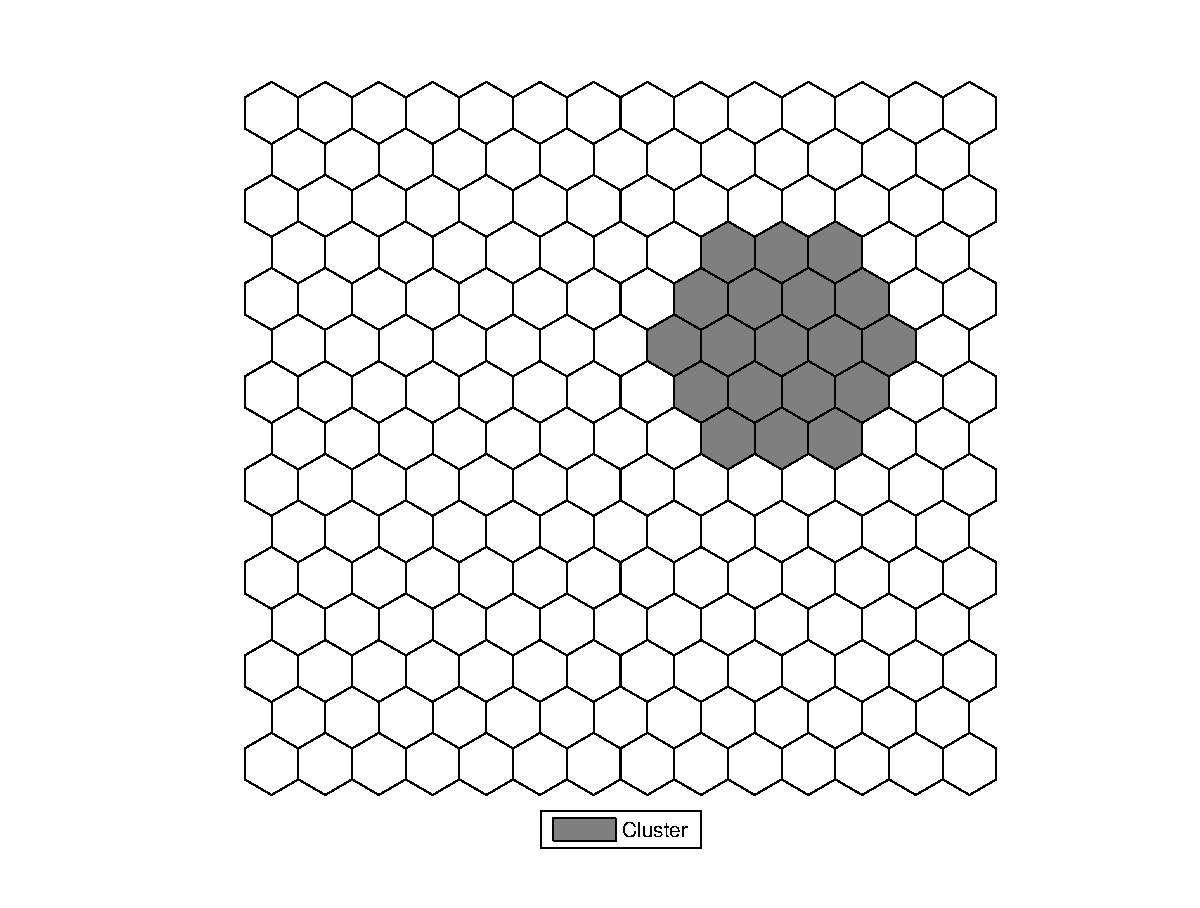
\includegraphics[width=0.38\textwidth, trim = 30 30 30 30]{cluster}
\end{figure}

\end{frame}

\section{Cronograma}

\begin{frame}
\frametitle{Cronograma}

Atividades a serem desenvolvidas durante o trabalho de conclusão de curso:

\definecolor{midgray}{gray}{.5}
\def\tablename{Tabela }%
\begin{table}[!htbp]\scriptsize
\centering %\caption{Cronograma 1/2016}
\label{c1}
%\rotatebox{90}{
\begin{tabular}{|l|c|c|c|c|c|}
\hline
\multicolumn{1}{|c|}{\multirow{\textbf{Atividades}}}&\multicolumn{5}{c|}{2/2016}\\
& Ago & Set & Out & Nov & Dez  \\
\hline
Escolha do tema a ser abordado&\cellcolor{midgray}&&&&\\
\hline
Desenvolvimento da proposta de projeto&&\cellcolor{midgray}&&&\\
   \cline{1-6}
Entrega da proposta de projeto&&\cellcolor{midgray}&&&\\
\cline{1-6}
Revisão de literatura&&&\cellcolor{midgray}&\cellcolor{midgray}&\\
\cline{1-6}
Elaboração da apresentação da proposta&&&\cellcolor{midgray}&&\\
\cline{1-6}
Implementação&\cellcolor{midgray}&\cellcolor{midgray}&\cellcolor{midgray}&\cellcolor{midgray}&\cellcolor{midgray}\\
\cline{1-6}
Verificação de Modelos&&\cellcolor{midgray}&&&\\
\cline{1-6}
Elaboração do rel. parcial&&&\cellcolor{midgray}&&\\
\cline{1-6}
Entrega do rel. parcial ao Orientador(a)&&&\cellcolor{midgray}&&\\
\cline{1-6}
Correção do do relatório parcial&&&&\cellcolor{midgray}&\\
\cline{1-6}
Entrega do relatório parcial para a banca&&&&\cellcolor{midgray}&\\
\cline{1-6}
Preparação do Banco de Dados&&&&\cellcolor{midgray}&\cellcolor{midgray}\\
\cline{1-6}
Elaboração do relatório final&&&&\cellcolor{midgray}&\cellcolor{midgray}\\
\cline{1-6}
\hline
\end{tabular}%}
\end{table}


\end{frame}

\begin{frame}
\frametitle{Cronograma}


\definecolor{midgray}{gray}{.5}
\begin{table}[!htbp]\scriptsize
\centering %\caption{Cronograma 2/2016}
\label{c2}
%\rotatebox{90}{
\begin{tabular}{|l|c|c|c|c|c|c|c|}
\hline
\multicolumn{1}{|c|}{\multirow{\textbf{Atividades}}} &\multicolumn{6}{|c|}{1/2017}\\
\hlin
& Fev & Mar & Abr & Mai & Jun & Jul   \\\hline
Verificação de Modelos&&\cellcolor{midgray}&&&&\\
\cline{1-6}
\hline
Elaboração do relatório final&\cellcolor{midgray}&\cellcolor{midgray}&\cellcolor{midgray}&&&\\
\cline{1-7}
Entrega do rel. de av. do orientador&&&\cellcolor{midgray}&&&\\
\cline{1-7}
Entrega do rel. final ao  orientador&&&\cellcolor{midgray}&\cellcolor{midgray}&&\\
\cline{1-7}
Correção do relatório final&&&\cellcolor{midgray}&\cellcolor{midgray}&&\\
\cline{1-7}
Entrega do rel. final para a banca&&&&\cellcolor{midgray}&&\\
\cline{1-7}
Início das apres. orais dos trabalhos&&&\cellcolor{midgray}&\cellcolor{midgray}&&\\
\cline{1-7}
Apresentação em pôster&&&&\cellcolor{midgray}&\cellcolor{midgray}&\cellcolor{midgray}\\
\hline
\end{tabular}%}
\end{table}

\end{frame}

% ----------------- NOVO SLIDE --------------------------------
\section{Referências}

% --- O comando \allowframebreaks ---
% Se o conteúdo não se encaixa em um quadro, a opção allowframebreaks instrui 
% beamer para quebrá-lo automaticamente entre dois ou mais quadros,
% mantendo o frametitle do primeiro quadro (dado como argumento) e acrescentando 
% um número romano ou algo parecido na continuação.

\begin{frame}[allowframebreaks]{Referências}
\bibliography{abntex2-modelo-references}
\nocite{fernandes2012detecccao}
\end{frame}

% ----------------- FIM DO DOCUMENTO -----------------------------------------
\end{document}
